% ============================================================
%  chapter13_slides.tex  --  Chapter 13: Conjugation
%  Convex Analysis and Monotone Operator Theory in Hilbert Spaces, 2nd ed.
%  Bauschke & Combettes  --  CMS Books in Mathematics, Springer 2017
%
%  Compile:  pdflatex -interaction=nonstopmode chapter13_slides.tex   (twice)
% ============================================================
\documentclass[aspectratio=169,10pt]{beamer}

\usetheme{Madrid}
\usecolortheme{seahorse}

\usepackage{amsmath,amssymb,amsfonts}
\usepackage{bm}
\usepackage{graphicx}
\usepackage{booktabs}
\usepackage{listings}
\usepackage{xcolor}
\usepackage{microtype}

\graphicspath{{figures/}}

% ---- listings Python style ----
\lstdefinestyle{python}{
  language=Python,
  basicstyle=\ttfamily\scriptsize,
  numbers=left,
  numberstyle=\tiny\color{gray},
  stepnumber=1,
  numbersep=5pt,
  frame=single,
  backgroundcolor=\color{gray!7},
  keywordstyle=\color{blue!70!black}\bfseries,
  commentstyle=\color{green!50!black}\itshape,
  stringstyle=\color{orange!80!black},
  breaklines=true,
  showstringspaces=false,
  tabsize=2,
}

\setbeamertemplate{footline}[frame number]
\setbeamertemplate{navigation symbols}{}

% ---- shorthand ----
\newcommand{\R}{\mathbb{R}}
\newcommand{\Hil}{\mathcal{H}}
\newcommand{\Kil}{\mathcal{K}}
\newcommand{\inner}[2]{\langle #1 \mid #2 \rangle}
\newcommand{\norm}[1]{\lVert #1 \rVert}
\newcommand{\dom}{\operatorname{dom}}
\newcommand{\epi}{\operatorname{epi}}
\newcommand{\gra}{\operatorname{gra}}
\newcommand{\ran}{\operatorname{ran}}
\newcommand{\Fix}{\operatorname{Fix}}
\newcommand{\rec}{\operatorname{rec}}
\newcommand{\Id}{\operatorname{Id}}
\newcommand{\iotaC}{\iota_C}
\newcommand{\sigmaC}{\sigma_C}
\newcommand{\GammaZero}{\Gamma_0(\Hil)}
\newcommand{\Gammabig}{\Gamma(\Hil)}
\newcommand{\conj}[1]{#1^{*}}
\newcommand{\biconj}[1]{#1^{**}}

% ============================================================
\title[Convex Analysis \& MOT -- Ch.13]{Convex Analysis and Monotone Operator Theory in Hilbert Spaces}
\subtitle{Chapter 13: Conjugation}
\author{Based on Bauschke \& Combettes}
\institute{CMS Books in Mathematics, Springer, 2nd ed., 2017}
\date{}

% ============================================================
\begin{document}

\begin{frame}
  \titlepage
\end{frame}

\begin{frame}{Outline}
  \tableofcontents
\end{frame}

% ============================================================
\section{Setting the Stage}
% ============================================================

\begin{frame}{Why conjugation?}
  \textbf{Big picture.} Throughout Chapters 8--12 we described a convex
  function $f$ by its \emph{values} $f(x)$ at \emph{points} $x$. Conjugation
  gives us a completely different, and often more powerful, description:
  we describe $f$ by how it compares to \emph{every linear functional}
  $\inner{\cdot}{u}$.

  \bigskip
  \begin{block}{The one-sentence idea}
    $f^*(y)$ measures the largest gap between the linear function
    $\inner{y}{\cdot}$ and $f$ --- it encodes $f$ from the ``slope''
    perspective instead of the ``point'' perspective.
  \end{block}

  \bigskip
  This is the continuous analogue of describing a convex polygon either by
  its vertices (points) or by its edges/supporting half-planes (slopes).
  Conjugation is the single most important construction in the theory: it
  underlies duality (Ch.\ 15), subdifferentials (Ch.\ 16), and proximal
  algorithms used throughout convex optimization and monotone operator
  splitting.
\end{frame}

\begin{frame}{Notation you'll need}
  \begin{columns}[t]
    \begin{column}{0.5\textwidth}
      \begin{itemize}
        \item $\Hil, \Kil$: real Hilbert spaces
        \item $\inner{x}{y}$: inner product; $\norm{x}$: induced norm
        \item $f: \Hil \to [-\infty,+\infty]$: extended-real-valued function
        \item $\dom f = \{x : f(x) < +\infty\}$
        \item $\epi f = \{(x,\xi)\in\Hil\times\R : f(x)\le \xi\}$: epigraph
        \item $f$ \emph{proper}: $f \not\equiv +\infty$ and $f > -\infty$
        \item $\Gammabig$: lower semicontinuous (lsc) convex functions
          $\Hil\to\,]-\infty,+\infty]$
        \item $\GammaZero$: \emph{proper} members of $\Gammabig$
      \end{itemize}
    \end{column}
    \begin{column}{0.5\textwidth}
      \begin{itemize}
        \item $\iotaC$: indicator function of $C$ ($0$ on $C$, $+\infty$
          off $C$)
        \item $\sigmaC = \conj{(\iotaC)}$: support function of $C$
        \item $q = \tfrac12\norm{\cdot}^2$
        \item $f\,\square\,g$: infimal convolution,
          $(f\square g)(x)=\inf_y (f(y)+g(x-y))$
        \item $\bar f$: lsc hull (closure) of $f$; $\breve f$: convex lsc
          hull of $f$
        \item $B(0;\rho)$: closed ball of radius $\rho$ about $0$
        \item $K^{\ominus}$: polar cone of $K$; $V^{\perp}$: orthogonal
          complement
        \item $\mathcal B(\Hil,\Kil)$: bounded linear operators $\Hil\to\Kil$
      \end{itemize}
    \end{column}
  \end{columns}
\end{frame}

% ============================================================
\section{13.1 Definition and Examples}
% ============================================================

\begin{frame}{Definition 13.1: the Fenchel conjugate}
  \textbf{Intuition.} For a fixed ``slope'' (vector) $u\in\Hil$, compare the
  linear function $x\mapsto\inner{x}{u}$ against $f$ everywhere, and record
  the \emph{largest} amount by which the linear function can exceed $f$.
  That largest gap, as a function of $u$, is the conjugate.

  \begin{block}{Definition (Fenchel conjugate)}
    Let $f : \Hil \to [-\infty,+\infty]$. The \emph{conjugate} of $f$ is the
    function $\conj f : \Hil \to [-\infty,+\infty]$ defined by
    \[
      \conj f(u) \;=\; \sup_{x\in\Hil}\big(\inner{x}{u} - f(x)\big).
      \tag{13.1}
    \]
    Here $u$ ranges over $\Hil$ (thought of as the space of ``slopes''),
    and the supremum is over all points $x$ where we test $f$ against the
    linear functional $\inner{\cdot}{u}$.
  \end{block}

  \medskip
  Equivalently (Proposition 13.10(iv)): restricting the supremum to
  $\dom f$, $\ \conj f(u) = \sup_{x\in\dom f}(\inner{x}{u}-f(x)) =
  \sup_{(x,\xi)\in\epi f}(\inner{x}{u}-\xi)$.
\end{frame}

\begin{frame}{Geometric picture (Fig.\ 13.1)}
  \begin{center}
    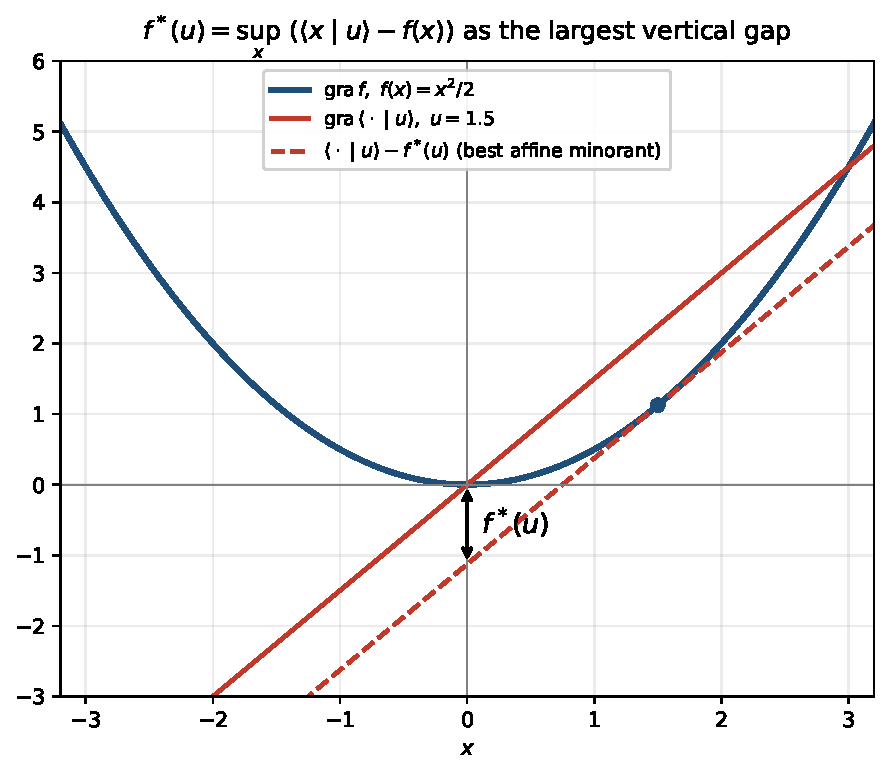
\includegraphics[width=0.72\linewidth]{fig_geometric_conjugate.pdf}
  \end{center}
  \textbf{Reading the picture.} The straight line $\gra\inner{\cdot}{u}$ is
  slid downward until it just touches $\gra f$ from below; the amount it
  had to move down is exactly $\conj f(u)$. Equivalently, $\conj f(u)$ is
  the vertical distance, measured at $x=0$, between the line
  $\inner{\cdot}{u}$ and the \emph{best affine minorant of $f$ with slope
  $u$}, namely $x\mapsto \inner{x}{u}-\conj f(u)$.
\end{frame}

\begin{frame}{Derivation 1/2: conjugate of $f(x)=x^2/2$ (self-duality)}
  \textbf{Setup.} $\Hil=\R$, $f(x) = x^2/2 = q(x)$.

  \textbf{Step 1 (write the sup).}
  \[
    \conj f(u) = \sup_{x\in\R}\Big(ux - \tfrac12 x^2\Big).
  \]
  \textbf{Step 2 (optimize over $x$).} The map $x\mapsto ux-\tfrac12 x^2$ is
  concave and differentiable; set the derivative to zero:
  \[
    \frac{d}{dx}\Big(ux-\tfrac12 x^2\Big) = u - x = 0 \;\Longrightarrow\; x^\star = u.
  \]
  \textbf{Step 3 (plug back in).}
  \[
    \conj f(u) = u\cdot u - \tfrac12 u^2 = \tfrac12 u^2.
  \]
  \begin{alertblock}{Conclusion: self-conjugacy}
    $\conj f(u) = \tfrac12 u^2 = f(u)$ for every $u$, i.e.\ $f^{*}=f$. This
    is Example 13.6 and is a special case of Proposition 13.19: among all
    functions on $\Hil$, $q=\tfrac12\norm{\cdot}^2$ is the \emph{only} one
    equal to its own conjugate.
  \end{alertblock}
\end{frame}

\begin{frame}{Derivation 2/2: conjugate of $f(x)=|x|$}
  \textbf{Setup.} $\Hil=\R$, $f(x)=|x|$.

  \textbf{Step 1 (write the sup).}
  \[
    \conj f(u) = \sup_{x\in\R}\big(ux - |x|\big).
  \]
  \textbf{Step 2 (split by sign of $x$).} For $x>0$: $ux-x = x(u-1)$; for
  $x<0$: $ux+x=x(u+1)$. Each is linear in $x$, so:
  \begin{itemize}
    \item If $|u|\le 1$: both slopes $u-1\le0$ and $u+1\ge 0$ push the
      supremum to $x=0$, giving value $0$.
    \item If $u>1$: letting $x\to+\infty$ makes $x(u-1)\to+\infty$.
    \item If $u<-1$: letting $x\to-\infty$ makes $x(u+1)\to+\infty$
      (since $u+1<0$ and $x\to-\infty$).
  \end{itemize}
  \textbf{Step 3 (assemble).}
  \[
    \conj f(u) =
    \begin{cases}
      0, & |u|\le 1,\\
      +\infty, & |u|>1.
    \end{cases}
    = \iota_{[-1,1]}(u).
  \]
  \begin{alertblock}{Conclusion}
    $\conj{|\cdot|} = \iota_{[-1,1]}$: the conjugate of the ``kinked'' norm
    on $\R$ is the indicator of the interval $[-1,1]$ (matches Example
    13.3(v) in $\Hil=\R$, where $\conj{\norm{\cdot}}=\iota_{B(0;1)}$).
  \end{alertblock}
\end{frame}

\begin{frame}{Figure: $f=|\cdot|$ and its conjugate side by side}
  \begin{center}
    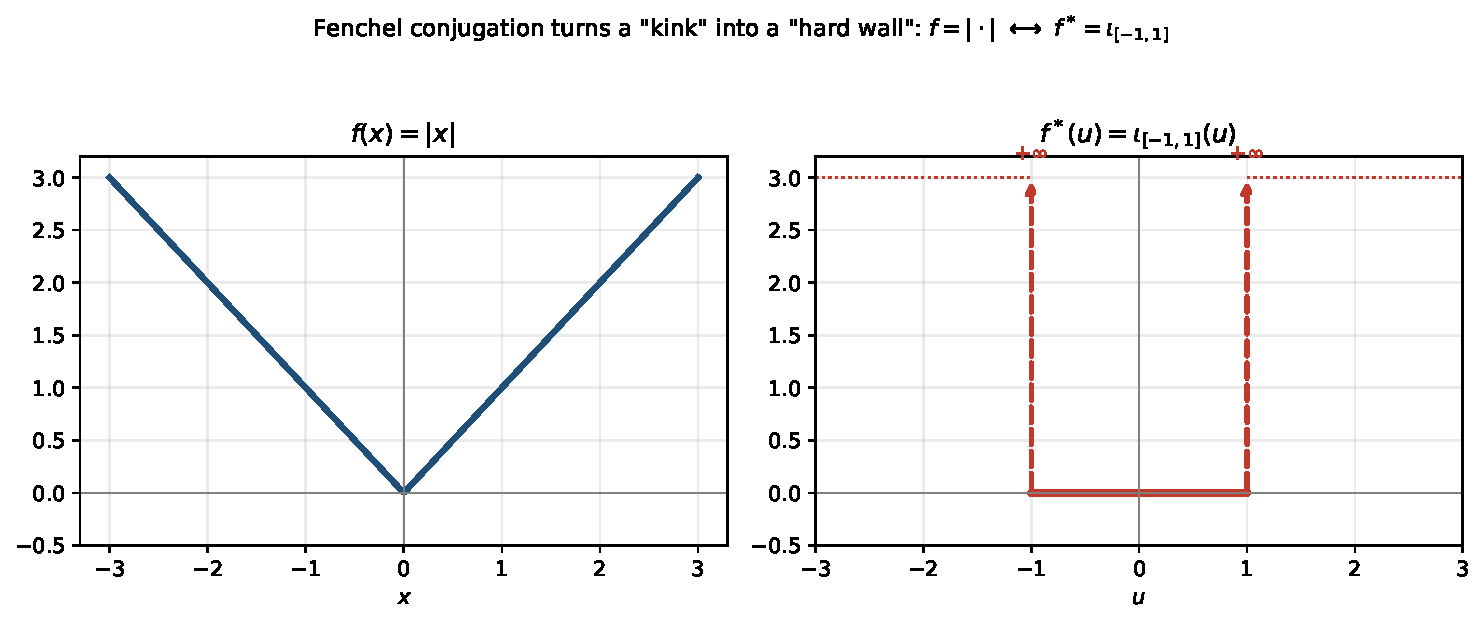
\includegraphics[width=0.92\linewidth]{fig_abs_and_conjugate.pdf}
  \end{center}
  Conjugation converts the single kink of $|x|$ at $0$ into a ``hard wall''
  at $u=\pm1$: any slope with $|u|>1$ can beat $f$ by an unbounded amount,
  while any slope with $|u|\le 1$ can never beat it at all.
\end{frame}

\begin{frame}{Running numeric example}
  \textbf{$f(x)=x^2/2$, using $\conj f(u)=u^2/2$:}
  \begin{center}
  \begin{tabular}{c|cccc}
    $u$ & $0$ & $1$ & $2$ & $-3$ \\ \hline
    $\conj f(u) = u^2/2$ & $0$ & $0.5$ & $2$ & $4.5$
  \end{tabular}
  \end{center}

  \bigskip
  \textbf{$f(x)=|x|$, using $\conj f(u)=\iota_{[-1,1]}(u)$:}
  \begin{center}
  \begin{tabular}{c|ccccc}
    $u$ & $0$ & $0.5$ & $1$ & $1.5$ & $-2$ \\ \hline
    $\conj f(u)$ & $0$ & $0$ & $0$ & $+\infty$ & $+\infty$
  \end{tabular}
  \end{center}

  \medskip
  Check Fenchel--Young (Proposition 13.15) at $x=1,u=2$ for $f=|\cdot|$:
  $f(1)+\conj f(2) = 1 + \infty \ge \inner{1}{2}=2$. Equality would require
  $x=1$ to attain the sup defining $\conj f(2)$; since $\conj f(2)=+\infty$
  and $f(1)=1$ is finite, the inequality is strict but trivially true.
\end{frame}

\begin{frame}{Example 13.2: a gallery of conjugates (I)}
  \textbf{Intuition.} Many named functions in information theory and
  statistics (negative entropies, log-barriers) are conjugates of
  elementary functions -- this is why conjugation shows up throughout
  optimization and statistical estimation.
  \begin{block}{Selected pairs $(f,\conj f)$ on $\R$}
    \begin{itemize}
      \item $f(x)=1/x$ on $\R_{++}$, $+\infty$ else $\;\Longrightarrow\;$
        $\conj f(u) = -2\sqrt{-u}$ for $u\le 0$, $+\infty$ for $u>0$.
      \item $f(x)=-\ln(x)$ on $\R_{++}$ (negative Burg entropy)
        $\;\Longrightarrow\;$ $\conj f(u) = -\ln(-u)-1$ for $u<0$,
        $+\infty$ for $u\ge0$.
      \item $\cosh^{*}(u) = u\,\mathrm{arcsinh}(u)-\sqrt{u^2+1}$.
      \item $\exp^{*}(u) = u\ln(u)-u$ for $u>0$; $0$ at $u=0$; $+\infty$
        for $u<0$ (negative Boltzmann--Shannon entropy).
    \end{itemize}
  \end{block}
\end{frame}

\begin{frame}{Example 13.2: a gallery of conjugates (II)}
  \begin{block}{More entropy-type pairs}
    \begin{itemize}
      \item Negative Fermi--Dirac entropy
        $f(x)=x\ln x+(1-x)\ln(1-x)$ on $]0,1[$ (with $f=0$ at $\{0,1\}$,
        $+\infty$ else) has $\conj f(u)=\ln(1+e^u)$; the ``flip''
        $(\conj f)^{\vee}$ is the \emph{logistic loss}.
      \item Negative Bose--Einstein entropy
        $f(x)=x\ln x-(x+1)\ln(x+1)$ on $\R_{++}$ has
        \[
          \conj f(u) = \begin{cases} -\ln(1-e^u), & u<0,\\ +\infty, & u\ge 0.\end{cases}
        \]
      \item $f(x)=\sqrt{1+x^2}$ has $\conj f(u) = -\sqrt{1-u^2}$ for
        $|u|\le1$, $+\infty$ for $|u|>1$.
    \end{itemize}
  \end{block}
  These all follow the same recipe as our two derivations: write the sup,
  differentiate (or bound), solve, and check the domain of validity.
\end{frame}

\begin{frame}{Example 13.3: conjugates of sets and cones}
  \textbf{Intuition.} Indicator functions convert set geometry into
  function language; their conjugates are exactly the classical support
  functions and polars from Chapter 7.
  \begin{block}{Direct applications of (13.1)}
    \begin{itemize}
      \item $f=\iotaC$ for $C\subset\Hil$ $\;\Longrightarrow\;$
        $\conj f = \sigmaC$ (support function of $C$).
      \item $f=\iota_K$, $K$ a nonempty cone $\;\Longrightarrow\;$
        $\conj f = \sigma_K = \iota_{K^{\ominus}}$ ($K^{\ominus}$: polar
        cone).
      \item $f=\iota_V$, $V$ a linear subspace $\;\Longrightarrow\;$
        $\conj f = \iota_{V^{\ominus}} = \iota_{V^{\perp}}$.
      \item $f=\iota_{B(0;1)}$ $\;\Longrightarrow\;$
        $\conj f = \sigma_{B(0;1)} = \norm{\cdot}$.
      \item $f=\norm{\cdot}$ $\;\Longrightarrow\;$ $\conj f = \iota_{B(0;1)}$
        (the $\Hil=\R$ instance of this is exactly our derivation of
        $\conj{|\cdot|}$ above!).
    \end{itemize}
  \end{block}
\end{frame}

\begin{frame}{Examples 13.4--13.9: quadratic perturbations}
  \textbf{Intuition.} Adding a scaled quadratic $\gamma^{-1}q$ to $\varphi$
  before conjugating produces a clean transformation rule --- this is the
  seed of the \emph{Moreau envelope} machinery used later in the book.
  \begin{block}{Quadratic perturbation formula (Example 13.4)}
    Let $\varphi$ be proper, $\gamma\in\R_{++}$, $f=\varphi+\gamma^{-1}q$. Then
    \[
      \conj f = \gamma q - {}^{\gamma}\!\varphi\circ\gamma\Id
              = \gamma q - \big(\varphi\,\square\,(\gamma^{-1}q)\big)\circ\gamma\Id,
      \tag{13.4}
    \]
    where ${}^{\gamma}\varphi = \gamma\,\varphi(\cdot/\gamma)$ is the
    \emph{epi-multiple} of $\varphi$ by $\gamma$.
  \end{block}
  \textbf{Consequences.}
  \begin{itemize}
    \item $f=\iotaC+q/2 \Rightarrow \conj f = (\norm{\cdot}^2-d_C^2)/2$
      (Example 13.5); with $C=\Hil$ this again gives self-conjugacy of $q$.
    \item $f=\iota_{B(0;\rho)}+q/2$: $\conj f(u)=\rho\norm u-\rho^2/2$ for
      $\norm u>\rho$, $\norm u^2/2$ for $\norm u\le\rho$ -- the
      \emph{Huber function} in $\R$ (Example 13.7).
  \end{itemize}
\end{frame}

% ============================================================
\section{13.2 Basic Properties}
% ============================================================

\begin{frame}{Proposition 13.10: first consequences of the definition}
  \textbf{Intuition.} Before deriving anything deep, record the ``free''
  facts that fall directly out of (13.1).
  \begin{block}{Basic facts}
    \begin{enumerate}
      \item[(i)] $\conj f(0) = -\inf f(\Hil)$.
      \item[(ii)] $-\infty\in \conj f(\Hil) \iff f\equiv+\infty \iff
        \conj f\equiv-\infty$.
      \item[(iii)] If $\conj f$ is proper, then $f$ is proper.
      \item[(iv)] $\conj f(u) = \sup_{x\in\dom f}(\inner xu - f(x))
        = \sup_{(x,\xi)\in\epi f}(\inner xu-\xi)$.
      \item[(v)] $\conj f = \iota^{*}_{\epi f}(\cdot,-1) = \sigma_{\epi f}(\cdot,-1)$.
      \item[(vi)] If $f$ is proper, $\conj f = \iota^{*}_{\gra f}(\cdot,-1)
        = \sigma_{\gra f}(\cdot,-1)$.
    \end{enumerate}
  \end{block}
  Item (i) already tells you $\conj f(0)$ for free: e.g.\ for $f(x)=x^2/2$,
  $\conj f(0)=-\inf f(\R) = 0 = f(0)$, consistent with self-conjugacy.
\end{frame}

\begin{frame}{Affine minorants $\leftrightarrow$ points of $\epi \conj f$}
  \begin{block}{Proposition 13.12}
    Let $f:\Hil\to[-\infty,+\infty]$. Then:
    \begin{enumerate}
      \item[(i)] $(u,\mu)\in\epi \conj f \iff \inner{\cdot}{u}-\mu \le f$.
      \item[(ii)] $\conj f\equiv+\infty$ iff $f$ has no continuous affine
        minorant.
      \item[(iii)] If $\dom\conj f\ne\varnothing$, then $f$ is bounded
        below on every bounded subset of $\Hil$.
    \end{enumerate}
  \end{block}
  \textbf{Intuition.} This is the precise bridge between the ``slope''
  picture and the ``point'' picture: every point $(u,\mu)$ under the graph
  of $\conj f$ corresponds \emph{exactly} to a continuous affine function
  $\inner\cdot u - \mu$ lying entirely below $f$.
\end{frame}

\begin{frame}{Proposition 13.13: the conjugate is always nice}
  \begin{alertblock}{Key structural fact}
    For \emph{any} $f:\Hil\to[-\infty,+\infty]$ (not assumed convex or
    lsc!), the conjugate satisfies
    \[
      \conj f \in \Gammabig,
    \]
    i.e.\ $\conj f$ is always convex and lower semicontinuous.
  \end{alertblock}
  \textbf{Why.} By Proposition 13.10(iv), $\conj f$ is a pointwise supremum
  of the affine (hence lsc convex) functions
  $\big(\inner{x}{\cdot}-\xi\big)_{(x,\xi)\in\epi f}$, and a supremum of lsc
  convex functions is lsc and convex (Proposition 9.3). Conjugation is a
  ``convexifying, lower-semicontinuizing'' operation --- no matter how wild
  $f$ is.
\end{frame}

\begin{frame}{Proposition 13.15: the Fenchel--Young inequality}
  \textbf{Intuition.} Directly from the definition of a supremum,
  $\inner xu - f(x) \le \conj f(u)$ for every pair $(x,u)$ --- rearranged,
  this is the single most-used inequality in convex analysis.
  \begin{block}{Fenchel--Young inequality}
    Let $f:\Hil\to\,]-\infty,+\infty]$ be proper. Then
    \[
      (\forall x\in\Hil)(\forall u\in\Hil)\quad
      f(x) + \conj f(u) \;\ge\; \inner{x}{u}.
      \tag{13.10}
    \]
    \begin{itemize}
      \item $f(x)$: value of the primal function at $x$;
      \item $\conj f(u)$: value of the conjugate at $u$;
      \item $\inner xu$: the ``coupling'' between the two spaces.
    \end{itemize}
  \end{block}
  \textbf{Numeric check.} For $f=q$, $x=u=2$: $f(2)+\conj f(2)=2+2=4=
  \inner22$: \emph{equality} holds (self-conjugate case, always tight at
  $x^\star=u$). For $f=|\cdot|$, $x=2,u=2$: $f(2)+\conj f(2)=2+\infty\ge4$:
  inequality only, since $u=2\notin[-1,1]$.
\end{frame}

\begin{frame}{Proposition 13.16: biconjugation}
  \textbf{Intuition.} Conjugating twice can only make the function smaller
  or equal (a ``regularization''); conjugating three times is the same as
  conjugating once.
  \begin{block}{Biconjugate facts}
    \begin{enumerate}
      \item[(i)] $\biconj f \le f$ always.
      \item[(ii)] $f\le g \Rightarrow \conj f\ge \conj g$ and
        $\biconj f \le \biconj g$ (conjugation reverses order).
      \item[(iii)] $f^{***} = \conj f$.
      \item[(iv)] $\conj{(\breve f)} = \conj f$ ($\breve f$: convex lsc
        hull of $f$).
    \end{enumerate}
  \end{block}
  \textbf{Warning (Example 13.17).} These inequalities can be extreme: for
  $f(x)=-|x|$ on $\R$, the convex hull $\breve f\equiv-\infty$ and
  $\conj f\equiv+\infty$ everywhere --- conjugation of a concave-looking
  function destroys all information.
\end{frame}

\begin{frame}{Proposition 13.19: Self-conjugacy is rigid}
  \begin{alertblock}{Self-conjugacy}
    \[
      f = \conj f \quad\Longleftrightarrow\quad f = \tfrac12\norm{\cdot}^2 = q.
    \]
  \end{alertblock}
  \textbf{Proof sketch.} ($\Leftarrow$) is Example 13.6. ($\Rightarrow$): if
  $f=\conj f$ then $f$ is proper (Prop.\ 13.10(ii)), and Fenchel--Young
  gives $2f(x)\ge\inner xx$, i.e.\ $f\ge q$; applying (13.16)(ii) to $f\ge
  q$ gives $\conj f \le \conj q = q$, i.e.\ $q\ge \conj f = f \ge q$, so
  $f=q$.

  \medskip
  \textbf{Consequence (Remark 13.20).} A convex cone $K\ne\Hil$ can never
  be self-polar in the strong sense $\iota_K = \iota_K^{*}$, because that
  would force $\iota_K=q$, impossible for an indicator function. In
  particular a linear subspace can never be self-orthogonal.

  \medskip
  This is exactly why our two running examples are so instructive: $q$
  is the \emph{unique} fixed point of conjugation, while $|\cdot|$ is very
  much \emph{not} one ($\conj{|\cdot|}=\iota_{[-1,1]}\ne|\cdot|$).
\end{frame}

\begin{frame}{Symmetry and scaling rules (Props.\ 13.21--13.23)}
  \begin{block}{Useful calculus rules}
    \begin{itemize}
      \item If $f$ is even, then $\conj f$ is even (Prop.\ 13.21).
      \item If $f\ge f(0)=0$, then $\conj f\ge \conj f(0)=0$ (Prop.\ 13.22).
      \item For $\alpha\in\R_{++}$: $(\alpha f)^{*}=\alpha f^{*}(\cdot/\alpha)$
        and $(\alpha f(\cdot/\alpha))^{*} = \alpha \conj f$ (Prop.\ 13.23(i)-(ii)).
      \item Translation: $(\tau_y f + \inner\cdot v+\beta)^{*} = \tau_v
        \conj f + \inner y\cdot - \inner yv - \beta$ (Prop.\ 13.23(iii)).
      \item Bijective $L\in\mathcal B(\Hil)$: $(f\circ L)^{*} = \conj f\circ
        L^{*-1}$ (Prop.\ 13.23(iv)).
    \end{itemize}
  \end{block}
  \textbf{Sanity check with our example.} $f=|\cdot|$, $\alpha=2$:
  $(2|\cdot|)^{*}(u) = 2\iota_{[-1,1]}(u/2) = 2\iota_{[-2,2]}(u) =
  \iota_{[-2,2]}(u)$ (indicator is $\{0,\infty\}$-valued, so the ``$2\times$''
  in front does not change the values --- only the set changed, from
  $[-1,1]$ to $[-2,2]$, exactly as scaling the slope threshold predicts.
\end{frame}

\begin{frame}{Proposition 13.24: infimal convolution $\leftrightarrow$ sum}
  \textbf{Intuition.} This is the single most important calculus rule for
  conjugates: it says that ``inf-convolving'' in the primal space
  corresponds \emph{exactly} to adding in the conjugate (dual) space.
  \begin{block}{Key duality formula}
    \[
      (f\,\square\,g)^{*} = \conj f + \conj g.
      \tag{13.17}
    \]
    Here $f\square g$ is the infimal convolution
    $(f\square g)(x)=\inf_{y\in\Hil}\big(f(y)+g(x-y)\big)$: it is the
    function-space analogue of Minkowski-summing epigraphs. If $f,g$ are
    proper, then also $(f+g)^{*} \le \conj f\,\square\,\conj g$
    (Prop.\ 13.24(ii)) --- equality generally requires a qualification
    condition (developed in Ch.\ 15).
  \end{block}
  \textbf{Also in Prop.\ 13.24:} $({}^{\gamma}f)^{*} = \conj f +
  (\gamma/2)\norm{\cdot}^2$; for $L\in\mathcal B(\Hil,\Kil)$,
  $(L\triangleright f)^{*} = \conj f\circ L^{*}$ (image/epi-composition
  rule) and $(f\circ L)^{*}\le L^{*}\triangleright \conj f$.
\end{frame}

\begin{frame}{Propositions 13.28--13.30: families and direct sums}
  \begin{block}{Infima/suprema of families}
    For a family $(f_i)_{i\in I}$ of proper functions:
    \begin{itemize}
      \item $\big(\inf_{i\in I} f_i\big)^{*} = \sup_{i\in I}\conj{f_i}$
        (Prop.\ 13.28(i), \emph{exact} equality).
      \item $\big(\sup_{i\in I} f_i\big)^{*} \le \inf_{i\in I}\conj{f_i}$
        (Prop.\ 13.28(ii), only $\le$ in general; with a sharpening to
        $\breve{(\cdot)}$ once all $f_i\in\Gamma_0$, Prop.\ 13.47).
    \end{itemize}
  \end{block}
  \begin{block}{Separable sums (Prop.\ 13.30)}
    For a finite family of Hilbert spaces $\Hil_i$ and functions $f_i$,
    \[
      \Big(\bigoplus_{i\in I} f_i\Big)^{*} = \bigoplus_{i\in I}\conj{f_i}.
      \tag{13.25}
    \]
    Conjugation of a ``block-separable'' function is just the
    block-separable conjugation of each piece --- e.g.\ this is exactly how
    Example 13.31 derives $\big((1/p)\norm\cdot_p^p\big)^{*} =
    (1/p^{*})\norm\cdot_{p^{*}}^{p^{*}}$ ($1/p+1/p^{*}=1$) in $\R^N$, and
    Example 13.32 derives $\norm\cdot_p^{*} = \iota_{B_{p^{*}}}$, i.e.\
    the classical $\ell_p$--$\ell_{p^{*}}$ duality via H\"older's inequality.
  \end{block}
\end{frame}

\begin{frame}{Bivariate functions and autoconjugacy (13.33--13.36)}
  \textbf{Intuition.} Conjugation extends naturally to functions of two
  Hilbert-space variables; ``marginalizing'' one variable before or after
  conjugating commute in a controlled way.
  \begin{block}{Proposition 13.33}
    Let $F:\Hil\times\Kil\to\,]-\infty,+\infty]$ be proper and set
    $f(x)=\inf_{y\in\Kil}F(x,y)$. Then $\conj f = \conj F(\cdot,0)$: the
    conjugate of a marginal is the conjugate evaluated at the dual variable
    of the marginalized coordinate set to $0$.
  \end{block}
  \begin{block}{Definition 13.34 (autoconjugate)}
    $F:\Hil\times\Hil\to[-\infty,+\infty]$ is \emph{autoconjugate} if
    $\conj F = F^{\intercal}$, where $F^{\intercal}(u,x)=F(x,u)$ (swap the
    two arguments). Proposition 13.36: if $F\in\Gamma(\Hil\oplus\Hil)$ is
    autoconjugate, then $F\ge\inner\cdot\cdot$ and $\conj F\ge\inner\cdot\cdot$.
  \end{block}
\end{frame}

% ============================================================
\section{13.3 The Fenchel--Moreau Theorem}
% ============================================================

\begin{frame}{Theorem 13.37: the Fenchel--Moreau theorem}
  \textbf{Intuition.} We already know $\biconj f\le f$ always
  (Prop.\ 13.16(i)), with equality failing whenever $f$ is not itself
  convex and lsc. The Fenchel--Moreau theorem says this is the \emph{only}
  obstruction: convexity + lower semicontinuity is exactly the property
  characterized by $f=\biconj f$.
  \begin{alertblock}{Theorem (Fenchel--Moreau)}
    Let $f:\Hil\to\,]-\infty,+\infty]$ be proper. Then
    \[
      f \text{ is lsc and convex} \quad\Longleftrightarrow\quad f = \biconj f.
    \]
    In this case, $\conj f$ is proper as well.
  \end{alertblock}
  \textbf{Why this matters.} It means $\GammaZero$ (proper lsc convex
  functions) is \emph{exactly} the set of functions that conjugation
  perfectly ``round-trips'' on. Conjugation is a genuine involution on
  $\GammaZero$, i.e.\ a duality --- not just a one-way transform.
\end{frame}

\begin{frame}{Proof sketch of Fenchel--Moreau}
  \textbf{($\Leftarrow$)} If $f=\biconj f$, then $f$ is a conjugate
  function, hence lsc and convex by Proposition 13.13. This direction is
  immediate.

  \medskip
  \textbf{($\Rightarrow$), main idea.} Suppose $f$ is lsc and convex. Fix
  $x\in\Hil$ and $\xi<f(x)$; project $(x,\xi)$ onto the closed convex set
  $\epi f$ to get $(p,\pi)$. The projection characterization
  (Proposition 9.18) forces $\pi\ge\xi$ and a separating-hyperplane-type
  inequality. Two cases:
  \begin{itemize}
    \item If $\pi>\xi$: setting $v=(x-p)/(\pi-\xi)$, one shows
      $\conj f(v)\le\inner xv-\pi$, hence $\biconj f(x)\ge\pi>\xi$.
    \item If $\pi=\xi$: a limiting argument using $w\in\dom \conj f$ and
      $\lambda\to+\infty$ shows $\biconj f(x)=+\infty=f(x)$ when
      $x\notin\dom f$, or $\biconj f(x)=f(x)$ when $x\in\dom f$.
  \end{itemize}
  Since $\xi<f(x)$ was arbitrary, $\biconj f(x)\ge f(x)$; combined with
  $\biconj f\le f$ always, we get $\biconj f = f$.
\end{frame}

\begin{frame}{Corollaries 13.38--13.42}
  \begin{block}{Immediate consequences}
    \begin{itemize}
      \item \textbf{Corollary 13.38.} $f\in\GammaZero \Rightarrow
        \conj f\in\GammaZero$ and $\biconj f=f$: conjugation is a bijection
        (in fact an involution) on $\GammaZero$.
      \item \textbf{Corollary 13.39.} For $f\in\GammaZero$:
        $f\le g \iff \conj f\ge \conj g$ (order-reversing bijection).
      \item \textbf{Corollary 13.40.} For $f,g\in\GammaZero$:
        $f=\conj g \iff g=\conj f$.
      \item \textbf{Corollary 13.42.} Every $f\in\GammaZero$ is the
        \emph{supremum of its continuous affine minorants} -- the
        continuous, affine version of ``every convex set is the
        intersection of its supporting half-spaces.''
    \end{itemize}
  \end{block}
  \textbf{Example 13.41.} Combining Example 13.32 with Corollary 13.40
  shows that the dual norm $\norm\cdot_{p,*}$ on $\R^N$ equals
  $\norm\cdot_{p^{*}}$: exactly the classical duality between $\ell_p$ and
  $\ell_{p^{*}}$ norms.
\end{frame}

\begin{frame}{Example 13.43: recovering old friends}
  Applying Fenchel--Moreau to specific indicator functions recovers
  familiar closure/polarity identities:
  \begin{block}{Consequences of $\biconj{(\iotaC)}=\iota_{\overline{\mathrm{conv}}\,C}$}
    \begin{itemize}
      \item $C\subset\Hil$ nonempty: $\iota_C^{**} = \iota_{\overline{\mathrm{conv}}\,C}$.
      \item $V$ a closed subspace: $\iota_V^{**}=\iota_V$, recovering
        $V^{\perp\perp}=V$.
      \item $K$ a nonempty closed convex cone: $\iota_K^{**}=\iota_K$,
        recovering $K^{\ominus\ominus}=K$ (bipolar theorem, Corollary
        6.34).
    \end{itemize}
  \end{block}
  This shows the abstract Fenchel--Moreau machinery reproduces very
  concrete geometric facts you already know from Chapters 3, 6, and 7.
\end{frame}

\begin{frame}{Propositions 13.44--13.46: lsc hulls}
  \textbf{Intuition.} What happens at a single point $x$ if $f$ is convex
  but \emph{not} lsc? Biconjugation still does something sensible: it
  computes the lsc hull.
  \begin{block}{Key equivalences (Prop.\ 13.44)}
    For $f$ convex with $f(x)\in\R$, the following are equivalent:
    (i) $f$ is lsc at $x$; (ii) $\biconj f(x)=\breve f(x)=\bar f(x)=f(x)$;
    (iii) $\biconj f(x)=f(x)$.
  \end{block}
  \begin{block}{Proposition 13.45 / 13.46}
    If $f$ has a continuous affine minorant, then $\biconj f = \breve f$
    (the lsc convex hull); otherwise $\biconj f\equiv-\infty$. For $f$
    proper convex with a continuous affine minorant: $\dom f\subset
    \dom\biconj f\subset\overline{\dom f}$, $\epi\biconj f=\overline{\epi f}$,
    and $\biconj f(x) = \varliminf_{y\to x} f(y)$.
  \end{block}
\end{frame}

\begin{frame}{Propositions 13.49--13.51: recession \& integral functionals}
  \begin{block}{Conjugates and recession functions (Prop.\ 13.49)}
    For $f\in\GammaZero$:
    \[
      \operatorname{rec}(\conj f) = \sigma_{\dom f}
      \qquad\text{and}\qquad
      \operatorname{rec} f = \sigma_{\dom \conj f}.
    \]
    The ``directions of recession'' of one function are governed by the
    support function of the \emph{domain} of the other.
  \end{block}
  \begin{block}{Conjugation of integral functionals (Prop.\ 13.50)}
    On $\Hil=L^2((\Omega,\mathcal F,\mu);\mathsf H)$, if
    $f(x)=\int_\Omega \varphi(x(\omega))\,\mu(d\omega)$ (an integral
    functional built from $\varphi\in\Gamma_0(\mathsf H)$), then under mild
    conditions $\conj f(u) = \int_\Omega \conj\varphi(u(\omega))\,\mu(d\omega)$:
    conjugation commutes with integration.
  \end{block}
  \textbf{Example 13.51.} For $X$ a square-integrable r.v.\ and
  $f(X)=\tfrac1p\mathsf E|X|^p$, we get $\conj f(X) = \tfrac1{p^{*}}
  \mathsf E|X|^{p^{*}}$: the $L^p$--$L^{p^{*}}$ duality for random variables.
\end{frame}

% ============================================================
\section{Computing Conjugates Numerically}
% ============================================================

\begin{frame}[fragile]{Python: conjugates via a discretized supremum}
  \textbf{Idea.} Since $\conj f(u) = \sup_{x}(ux-f(x))$, we can
  \emph{approximate} $\conj f$ on any finite grid of $u$-values by
  brute-force maximizing over a fine grid of $x$-values -- no closed form
  needed. This is exactly how one would numerically explore conjugates of
  functions too complicated to differentiate by hand.

  \begin{lstlisting}[style=python]
import numpy as np

def numerical_conjugate(f, x_grid, u_grid):
    """f*(u) = sup_x (u*x - f(x)), brute force over a grid."""
    fx = f(x_grid)                      # shape (len(x_grid),)
    # outer(u,x) - f(x): shape (len(u_grid), len(x_grid))
    vals = np.outer(u_grid, x_grid) - fx[None, :]
    return np.max(vals, axis=1)

x_grid = np.linspace(-8, 8, 4001)
u_grid = np.linspace(-2.5, 2.5, 400)

f_quad = lambda x: 0.5 * x**2          # self-conjugate
f_abs  = lambda x: np.abs(x)           # conjugate = indicator of [-1,1]

fstar_quad = numerical_conjugate(f_quad, x_grid, u_grid)
fstar_abs  = numerical_conjugate(f_abs,  x_grid, u_grid)

print(fstar_quad[u_grid == 1.5])   # ~1.125, matches u^2/2
print(fstar_abs[np.argmin(np.abs(u_grid-0.5))])   # ~0
print(fstar_abs[np.argmin(np.abs(u_grid-2.0))])   # large (approx +inf)
  \end{lstlisting}
\end{frame}

\begin{frame}{Numerical vs.\ analytic conjugates}
  \begin{center}
    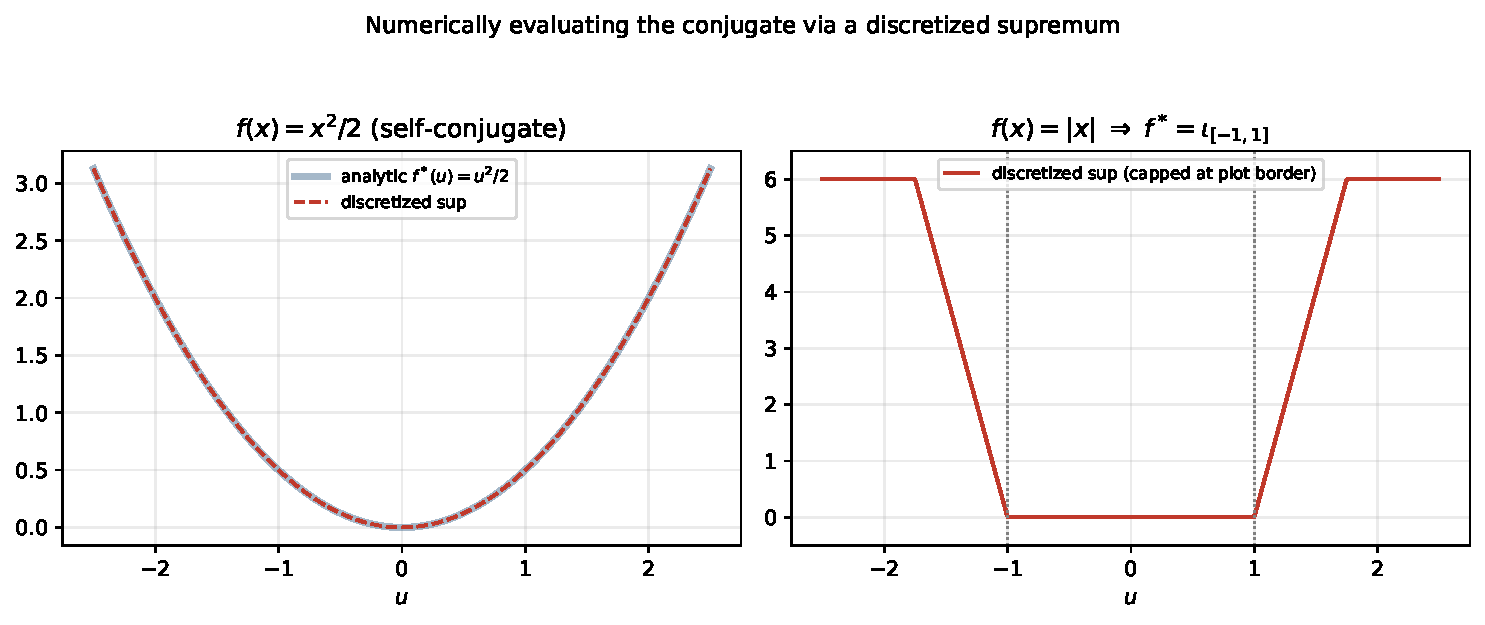
\includegraphics[width=0.95\linewidth]{fig_numeric_vs_analytic.pdf}
  \end{center}
  The discretized supremum recovers $\conj f(u)=u^2/2$ almost exactly for
  $f=q$ (a smooth, unconstrained optimization over $x$), while for
  $f=|\cdot|$ it correctly explodes as soon as $|u|$ exceeds $1$, saturating
  at the largest value $\max(u\cdot x)-|x|$ achievable on the finite
  $x$-grid --- a finite-grid stand-in for $+\infty$.
\end{frame}

% ============================================================
\section{Summary}
% ============================================================

\begin{frame}{Summary: Chapter 13 in one slide}
  \begin{itemize}
    \item \textbf{Definition.} $\conj f(u) = \sup_{x}(\inner xu - f(x))$:
      the largest gap between a linear functional and $f$.
    \item \textbf{Always true.} $\conj f\in\Gamma(\Hil)$ (convex, lsc), no
      matter what $f$ is; Fenchel--Young: $f(x)+\conj f(u)\ge\inner xu$.
    \item \textbf{Self-duality is rigid.} $f=\conj f$ forces
      $f=\tfrac12\norm\cdot^2$ (Prop.\ 13.19); e.g.\ $\conj{|\cdot|} =
      \iota_{[-1,1]} \ne |\cdot|$.
    \item \textbf{Biconjugation.} $\biconj f\le f$ always;
      \emph{Fenchel--Moreau}: equality holds iff $f$ is proper, lsc, and
      convex, and then $\conj f$ is proper too.
    \item \textbf{Calculus.} Inf-convolution $\leftrightarrow$ sum
      ($(f\square g)^{*}=\conj f+\conj g$); separable sums add
      coordinatewise; scaling/translation/linear-map rules all have clean
      conjugate analogues.
    \item \textbf{Where this leads.} Chapter 14 develops Moreau's
      decomposition and further conjugation identities; Chapter 15 builds
      Fenchel--Rockafellar duality directly on these tools.
  \end{itemize}
\end{frame}

\end{document}
